% =====================================================================
% Paper II  --  the announced sequel to "Random Signs into Matchings"
% (godsil-gutman-lean). Delivers the path-tree proposal of Paper I:
% a machine-checked Heilmann--Lieb theorem in Lean 4.
% Style: technical, unambiguous, story-driven (each section opens with a
% question), key formulas framed and centred. Honesty rules verbatim:
% "proven" = sorry-free; scope stated exactly; nothing hidden.
% Verified against the Lean source 2026-06-05 (lake build MSS, exit 0;
% #print axioms on the headline theorems -> propext, Classical.choice,
% Quot.sound only). Toolchain v4.30.0-rc2, local Mathlib.
% =====================================================================
\documentclass[11pt]{article}
\usepackage[T1]{fontenc}
\usepackage{lmodern}
\usepackage{amsmath,amssymb,amsthm,booktabs,graphicx,hyperref}
\usepackage{xurl}
\usepackage[table]{xcolor}
\definecolor{ggteal}{HTML}{1B6F8C}
\definecolor{ggband}{HTML}{DCE7EB}
\definecolor{ggamber}{HTML}{E08A1E}
\usepackage[margin=1in]{geometry}
\usepackage{microtype}
\usepackage[most]{tcolorbox}
\setlength{\emergencystretch}{6em}
\graphicspath{{figures/}}
\newtheorem{theorem}{Theorem}
\newtheorem{lemma}{Lemma}
\newtheorem{definition}{Definition}
\newcommand{\lean}[1]{{\def\_{\textunderscore\allowbreak}\texttt{#1}}}
\newcommand{\Z}{\mathbb{Z}}
\newcommand{\R}{\mathbb{R}}
\hypersetup{colorlinks=true,linkcolor=ggteal,citecolor=ggteal,urlcolor=ggteal}
% framed, centred display for the load-bearing formulas
\newtcbox{\keybox}{on line,boxrule=0.9pt,colframe=ggteal,colback=ggband!40,
  arc=3pt,left=8pt,right=8pt,top=5pt,bottom=5pt}
\newcommand{\keyeq}[1]{\begin{center}\keybox{$\displaystyle #1$}\end{center}}

\title{\bf Unfolding a Graph into a Tree\\[4pt]
  \large\normalfont A machine-checked proof of the Heilmann--Lieb theorem in Lean~4}
\author{Carles Mar\'in\thanks{Formalized with AI assistance (Claude, Anthropic); the mathematics and all claims are the author's responsibility. The methodology is discussed in Section~\ref{sec:method}.}\\[3pt]
  \normalsize Independent researcher\\
  \normalsize \texttt{karlesmarin@gmail.com}}
\date{June 2026}

\begin{document}
\maketitle

\begin{abstract}
This is the sequel promised at the end of \emph{Random Signs into
Matchings}~\cite{PartI}, where I formalized the Godsil--Gutman identity and the
matching polynomial in Lean~4 and proposed, as the next step, a proof of the
\emph{Heilmann--Lieb theorem} through Godsil's path tree. Here I carry out that
proposal in full. I report a machine-checked proof, \lean{sorry}-free, that the
matching polynomial $\mu_G(x)=\sum_k(-1)^k m_k\,x^{n-2k}$ of every finite graph is
real-rooted, and that---when the maximum degree satisfies $2\le\Delta$---all its
roots lie in the Ramanujan band $[-2\sqrt{\Delta-1},\,2\sqrt{\Delta-1}]$. The
proof follows Godsil exactly: unfold $G$ into the tree $T(G,u)$ of its paths, where
the matching polynomial equals a characteristic polynomial and the bound is a
spectral fact; transport back along the divisibility $\mu_G\mid\mu_{T(G,u)}$. I
build the path tree, prove the divisibility (crossing the single elaboration wall
that the path-tree draft of this program had stopped at), and prove the bound from
the ground up by a weighted Gershgorin estimate reduced to two facts about
distances in a tree. I am not aware of any prior formalization, in any proof
assistant, of either half of Heilmann--Lieb, or of the matching polynomial itself.
I am exact about the boundary: the bound genuinely needs $\Delta\ge2$ (I give the
$K_2$ counterexample), the proof is of classical mathematics and finds no new
theorem, and the novelty claim rests on a search of the major proof-assistant
ecosystems (Lean, Isabelle, Coq), not an exhaustive byte-level audit.
\end{abstract}

\noindent\emph{Reader's map.} If you read only one thing, read
Theorem~\ref{thm:HL} and Figure~\ref{fig:km}---the statement, and why
$2\sqrt{\Delta-1}$ is the number. The proof is a single journey: unfold the graph
into a tree (Figure~\ref{fig:pathtree}), bound the tree
(Sections~\ref{sec:gershgorin}--\ref{sec:weight}), and carry the bound home
(Figure~\ref{fig:nested}). The load-bearing facts are the framed identities; the
honest limits are stated as plainly as the results.

\begin{figure}[t]
  \centering
  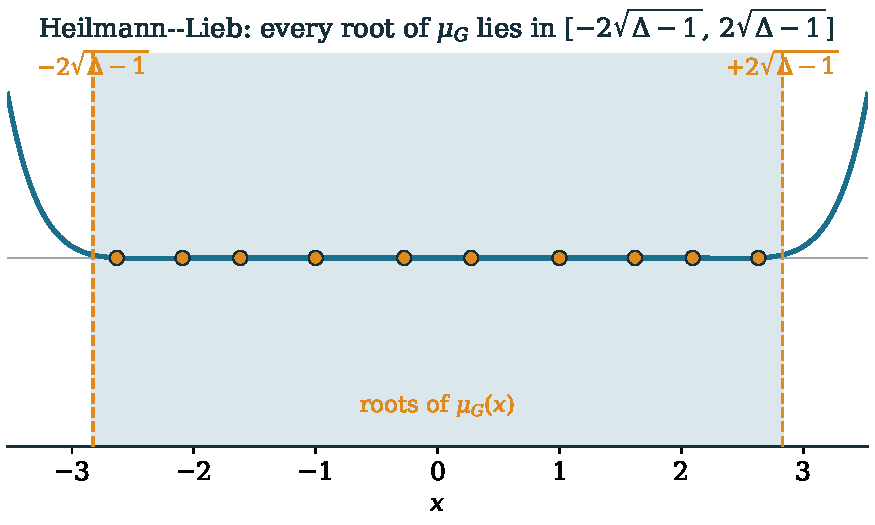
\includegraphics[width=0.92\textwidth]{fig1_band.pdf}
  \caption{The theorem, in one picture. The normalized matching polynomial
  $\mu_G$ of the Petersen graph ($\Delta=3$), with its roots (amber) and the
  Ramanujan band $[-2\sqrt{\Delta-1},2\sqrt{\Delta-1}]$ shaded. Heilmann--Lieb
  asserts---and \lean{matchingPoly\_bounded} now certifies---that the roots never
  leave the band, for every finite graph with $\Delta\ge2$.}
  \label{fig:band}
\end{figure}

% ===============================================================
\section{Introduction: a short history, and why this paper}
\label{sec:history}

\emph{Could a theorem born in the physics of 1972, given a purely combinatorial
proof in the 1980s and an unexpected starring role in 2015, finally be placed
beyond doubt by a machine---and what would that be good for?} That is the question
behind this paper, and answering it requires three threads of history to meet.

The first thread is \emph{statistical mechanics}. In 1972, studying monomer--dimer
systems---a lattice gas of non-overlapping dimers---Heilmann and
Lieb~\cite{HeilmannLieb1972} proved that the zeros of the associated partition
function avoid an entire region of the complex plane. Translated to combinatorics,
their result says that the \emph{matching polynomial}
$\mu_G(x)=\sum_k(-1)^k m_k x^{n-2k}$ of a graph has only real roots, and that those
roots are confined to the band $[-2\sqrt{\Delta-1},\,2\sqrt{\Delta-1}]$ set by the
maximum degree $\Delta$. The result belongs to the Lee--Yang tradition (1952) of
controlling a physical system by the location of its partition function's zeros;
Heilmann and Lieb's contribution was to pin those zeros to the real axis and a
finite interval. The theorem was born analytic, in physics, not in graph theory.

The second thread is \emph{combinatorics}. In the 1980s Godsil gave a proof with
no analysis at all~\cite{Godsil1981Matchings,Godsil1993}: \emph{unfold} the graph
$G$ into the tree $T(G,u)$ of its paths, where the matching polynomial coincides
with the characteristic polynomial of a symmetric matrix---so reality and the band
are spectral facts---and transport the conclusion back along the divisibility
$\mu_G\mid\mu_{T(G,u)}$. The band edge $2\sqrt{\Delta-1}$ is no accident: it is the
spectral radius of the infinite $\Delta$-regular tree, computed by Kesten (1959),
and it is the number that names the \emph{Ramanujan graphs}. Those optimal
expanders---non-trivial spectrum inside the band---were constructed by Lubotzky,
Phillips and Sarnak and by Margulis (1988), whose proof that the bound is attained
rested on the Ramanujan--Petersson conjecture (hence the name); Alon--Boppana then
showed the bound cannot be beaten asymptotically. Seen multiplicatively, the same
band is the critical line of the \emph{Ihara zeta function} of a graph (Ihara 1966;
Bass 1992): a regular graph is Ramanujan exactly when its zeta satisfies an
analogue of the Riemann hypothesis. One number, $2\sqrt{\Delta-1}$, threads
matchings, spectra and zeta functions together (Figure~\ref{fig:km}).

\begin{figure}[t]
  \centering
  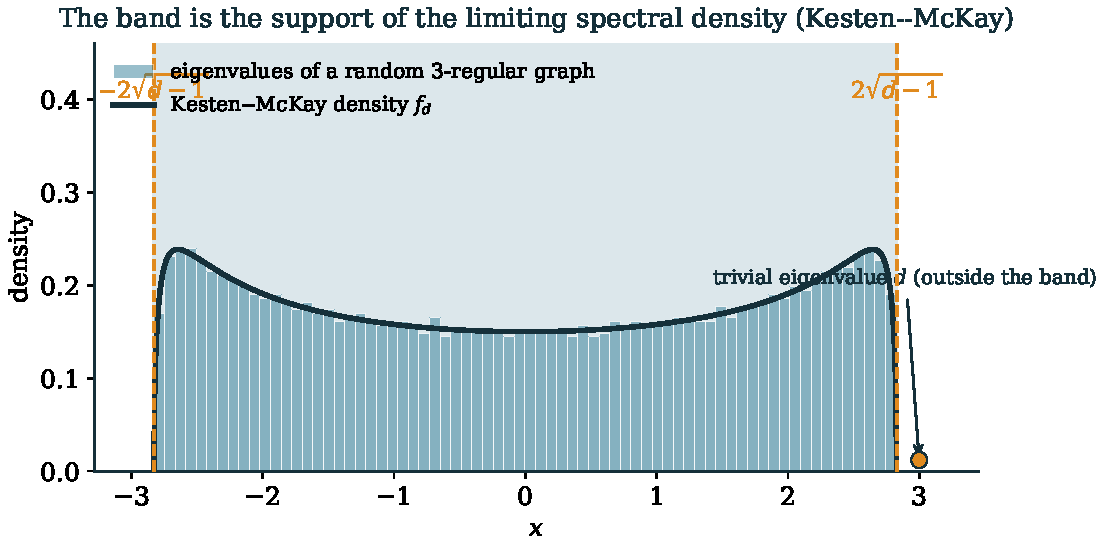
\includegraphics[width=0.9\textwidth]{fig6_kestenmckay.pdf}
  \caption{Why $2\sqrt{\Delta-1}$ is the right number. The eigenvalues of a random
  $3$-regular graph (teal) follow the Kesten--McKay limiting density (dark curve),
  and both live exactly on the band $[-2\sqrt{d-1},\,2\sqrt{d-1}]$: the density
  reaches the edges (amber) and vanishes beyond them. The lone trivial eigenvalue
  $d$ sits outside; a graph is \emph{Ramanujan} precisely when every non-trivial
  eigenvalue stays inside the band---the same band into which this paper confines
  the roots of the matching polynomial.}
  \label{fig:km}
\end{figure}

The third thread is \emph{theoretical computer science}. In 2015,
Marcus, Spielman and Srivastava~\cite{MSS2015a} proved that bipartite Ramanujan
graphs of every degree exist---resolving a long-standing question---and the
analytic engine of their argument is exactly Heilmann--Lieb: the expected
characteristic polynomial of a randomly signed adjacency matrix \emph{is} the
matching polynomial (Godsil--Gutman), and its roots lie in the band. A theorem
from lattice physics had become the keystone of a famous result about networks.

Against these three threads stands a fourth, younger one: the rise of
\emph{proof assistants}. Systems such as Lean and its library Mathlib now carry
machine-checked proofs of substantial modern mathematics. Yet---remarkably for a
theorem this central---neither the matching polynomial nor either half of
Heilmann--Lieb had been formalized in any proof assistant. Paper~I~\cite{PartI}
took the first step, formalizing the matching polynomial and the Godsil--Gutman
identity, and proposed Godsil's path tree as the route to the rest. \emph{This
paper walks that route to the end.} What the reader will find is a complete,
\lean{sorry}-free, machine-checked proof of both halves of Heilmann--Lieb, built
exactly along Godsil's unfolding, with the one elaboration wall that had stopped an
earlier draft now crossed.

Why it matters is the meeting of the threads. A verified Heilmann--Lieb is a
zero-free-region statement a statistical physicist can build on; the analytic input
an expander theorist needs, now beyond doubt; reusable real-rootedness and spectral
infrastructure for the formal-mathematics community; and a concrete stepping stone
toward a machine-checked proof that Ramanujan graphs exist.
Section~\ref{sec:implications} makes the reach across fields precise,
Section~\ref{sec:context} states plainly where the theorem stops being useful, and
Section~\ref{sec:open} leaves the sharpest unanswered questions on the table.

% ===============================================================
\section{The result}
\label{sec:intro}

So much for the map; here is the territory. Paper~I~\cite{PartI} ended on a promise
---\emph{``If this paper has a sequel, this is its first sentence.''}---and named the
route: prove Heilmann--Lieb not through interlacing machinery but through Godsil's
path tree, the one construction that yields both halves at once. This is that
sentence, and the rest of the paper keeps the promise.

The object of study is the \emph{matching polynomial} of a finite graph $G$ on $n$
vertices,
\keyeq{\mu_G(x)\;=\;\sum_{k\ge0}(-1)^k\,m_k\,x^{\,n-2k},}
where $m_k$ is the number of $k$-edge matchings of $G$ (and $m_0=1$). Heilmann and
Lieb~\cite{HeilmannLieb1972} proved two facts about its roots: they are all
\emph{real}, and they all lie in a band whose width is set by the maximum degree
$\Delta$ alone.

\begin{theorem}[Heilmann--Lieb, in Lean~4]
\label{thm:HL}
For every finite graph $G$, $\mu_G$ is real-rooted
(\lean{matchingPoly\_realRooted}); and if $2\le\Delta$ and every vertex has degree
$\le\Delta$, then every root of $\mu_G$ lies in the band
\keyeq{\bigl[-2\sqrt{\Delta-1},\;2\sqrt{\Delta-1}\bigr]\qquad
  (\lean{matchingPoly\_bounded}).}
Both statements are \lean{sorry}-free; \lean{\#print axioms} on each reports only
\lean{propext}, \lean{Classical.choice}, \lean{Quot.sound}.
\end{theorem}

Figure~\ref{fig:band} shows the conclusion; Table~\ref{tab:results} lists every
machine-checked ingredient; Table~\ref{tab:numeric} confirms the bound numerically
on six graphs.

\paragraph{The route, in one breath.}
A tree is easy: on a forest the matching polynomial \emph{equals} the
characteristic polynomial of the symmetric adjacency matrix, so it is real-rooted,
and the spectral radius of a tree of maximum degree $\Delta$ is at most
$2\sqrt{\Delta-1}$. Godsil's idea is to reduce the arbitrary graph to this easy
case by \emph{unfolding} it into the tree $T(G,u)$ of its paths and using the
divisibility
\keyeq{\mu_G \;\bigm|\; \mu_{T(G,u)}\qquad(\text{Godsil}),}
which transports any root bound on the tree back to $G$. Paper~I named exactly
these two facts---divisibility and the forest identity---as the work to do. This
paper does both, and proves the spectral bound on the tree from scratch.

\paragraph{Contributions.} All in Lean~4 / Mathlib, all \lean{sorry}-free
(Table~\ref{tab:results}):
\begin{enumerate}\itemsep2pt
\item \textbf{Real-rootedness} for every finite graph
  (\lean{matchingPoly\_realRooted}), via the path tree, its acyclicity, the forest
  identity, and the divisibility $\mu_G\mid\mu_{T(G,u)}$---the last of which
  required crossing an elaboration wall that an earlier draft of this program had
  diagnosed but not passed (Section~\ref{sec:divis}).
\item \textbf{The Ramanujan bound} for every finite graph with $\Delta\ge2$
  (\lean{matchingPoly\_bounded}), proved from the ground up by a weighted
  Gershgorin / Collatz--Wielandt estimate (Section~\ref{sec:gershgorin}) fed by a
  geometric tree weight and two facts about distances in a tree
  (Section~\ref{sec:weight}).
\item \textbf{Reusable infrastructure}: a hands-on weighted Gershgorin eigenvalue
  bound (\lean{collatzWielandt}); the \lean{BoundedBy} predicate closed under
  divisors and products; and two clean tree-distance facts. Mathlib had none of
  these, nor the matching polynomial (Paper~I).
\end{enumerate}

\paragraph{What I claim as new.} The mathematics is classical
(Section~\ref{sec:related}); the novelty lies in the formalization and in a few
things I had to build or find along the way. I claim, specifically:
\begin{enumerate}\itemsep1.5pt
\item[(N1)] the first machine-checked proof I am aware of, in any proof assistant,
  of \emph{both} halves of Heilmann--Lieb---real-rootedness and the Ramanujan
  bound---and of the matching polynomial they concern (search-based; see the caveat
  below);
\item[(N2)] a hands-on weighted Gershgorin eigenvalue bound \lean{collatzWielandt}
  and the \lean{BoundedBy} predicate closed under divisors and products
  (\lean{of\_dvd}, \lean{prod})---neither in Mathlib;
\item[(N3)] two reusable tree-distance lemmas---neighbours differ in root-distance
  by exactly one, and at most one neighbour is closer---proved respectively from
  bipartiteness and path-uniqueness;
\item[(N4)] the crossing of the elaboration wall that stopped the path-tree draft
  of this program, with the exact diagnosis (instance divergence over the
  $\Sigma$-paths type) and its cure (a head-pinned instance-irrelevance rewrite);
\item[(N5)] an edge-\emph{local} test weight that telescopes to the sharper
  per-edge bound $\sqrt{d_u-1}+\sqrt{d_v-1}$ and is the cleaner object to formalize;
\item[(N6)] a documented honest negative---the two-sided handle
  $\mathbb{E}[\operatorname{charpoly}(A_s^2)]$ is \emph{not} real-rooted---which
  closes one tempting route toward the open non-bipartite Ramanujan problem.
\end{enumerate}
I am careful about the kind of novelty: (N1)--(N4) are \emph{formalization}
contributions, (N5) a known-type bound I believe is first machine-checked, and
(N6) a negative result; none is new \emph{mathematics} in the theorem-proving
sense, and I separate them from the classical content deliberately.

\paragraph{And, plainly, what this is not.} It is a formalization of classical
mathematics; it proves no new theorem and claims none. The bound requires
$\Delta\ge2$ and I prove nothing weaker is needed by exhibiting where it fails
(Section~\ref{sec:weight}). And ``first formalization'' is supported by a search of
the three major proof-assistant ecosystems---Lean/Mathlib, the Isabelle Archive of
Formal Proofs, and Coq/mathcomp---none of which appears to contain the matching
polynomial or either half of Heilmann--Lieb (Mathlib has \lean{IsMatching} but no
matching polynomial). It is a search of catalogues and discussion archives, not a
byte-level audit of every library, so I state it as exactly that.

% Color tables for the Heilmann--Lieb (Paper II) document.
% Requires: \usepackage[table]{xcolor}; colors ggteal, ggband, ggamber defined in preamble.

\begin{table}[t]
\centering
\renewcommand{\arraystretch}{1.25}
\setlength{\tabcolsep}{7pt}
\rowcolors{2}{ggband}{white}
\begin{tabular}{@{}>{\raggedright\arraybackslash}p{0.345\textwidth} >{\raggedright\arraybackslash}p{0.46\textwidth} c@{}}
\rowcolor{ggteal}
\textcolor{white}{\bf Lean theorem} & \textcolor{white}{\bf Statement} & \textcolor{white}{\bf sorry-free} \\
\lean{matchingPoly\_realRooted} & $\mu_G$ is real-rooted, every finite $G$ & \checkmark \\
\lean{matchingPoly\_bounded} & roots of $\mu_G$ in $[-2\sqrt{\Delta-1},2\sqrt{\Delta-1}]$ ($2\le\Delta$, $\deg\le\Delta$) & \checkmark \\
\lean{connected\_matchingPoly\_dvd\_pathTree} & $\mu_G \mid \mu_{T(G,u)}$ (divisibility, brick) & \checkmark \\
\lean{matchingPoly\_forest\_eq\_charpoly} & $\mu_F=\operatorname{charpoly}(A_F)$ on a forest & \checkmark \\
\lean{collatzWielandt} & weighted Gershgorin eigenvalue bound & \checkmark \\
\lean{forest\_bounded\_proof} & forest matching roots in the band & \checkmark \\
\lean{forest\_adj\_dist\_pm\_one} & neighbours differ in root-distance by $1$ & \checkmark \\
\lean{forest\_le\_one\_parent} & $\le 1$ neighbour closer to the root & \checkmark \\
\lean{pathTree\_degree\_le} & $\deg T(G,u)\le \deg G$ & \checkmark \\
\end{tabular}
\caption{The machine-checked results of this paper, in Lean~4 / Mathlib. Every entry is
\lean{sorry}-free; \lean{\#print axioms} on each reports only \lean{propext},
\lean{Classical.choice}, \lean{Quot.sound} (no \lean{sorryAx}). Toolchain
\lean{leanprover/lean4:v4.30.0-rc2}, local Mathlib clone; verified \lean{lake build MSS} (exit~0).}
\label{tab:results}
\end{table}

\begin{table}[t]
\centering
\renewcommand{\arraystretch}{1.25}
\setlength{\tabcolsep}{9pt}
\rowcolors{2}{ggband}{white}
\begin{tabular}{@{}l c c c c c@{}}
\rowcolor{ggteal}
\textcolor{white}{\bf graph $G$} & \textcolor{white}{$n$} & \textcolor{white}{$\Delta$} &
\textcolor{white}{$2\sqrt{\Delta-1}$} & \textcolor{white}{$\max_i|\rho_i|$} & \textcolor{white}{in band} \\
path $P_6$       & 6 & 2 & 2.0000 & 1.8019 & \checkmark \\
cycle $C_6$      & 6 & 2 & 2.0000 & 1.9319 & \checkmark \\
star $K_{1,5}$   & 6 & 5 & 4.0000 & 2.2361 & \checkmark \\
complete $K_5$   & 5 & 4 & 3.4641 & 2.8570 & \checkmark \\
Petersen         & 10 & 3 & 2.8284 & 2.6314 & \checkmark \\
$3$-cube $Q_3$   & 8 & 3 & 2.8284 & 2.5779 & \checkmark \\
\end{tabular}
\caption{Numerical confirmation of the bound (\lean{matchingPoly\_bounded}). For each graph,
$\Delta$ is the maximum degree, $2\sqrt{\Delta-1}$ the Ramanujan band edge, and
$\max_i|\rho_i|$ the largest magnitude among the (exactly computed) roots $\rho_i$ of $\mu_G$.
Every value satisfies $\max_i|\rho_i|\le 2\sqrt{\Delta-1}$. Computed in SageMath.}
\label{tab:numeric}
\end{table}


% ===============================================================
\section{What is the path tree?}
\label{sec:pathtree}

How can a statement about an \emph{arbitrary} graph---with all its cycles---be
reduced to a statement about trees? Godsil's answer is to replace $G$ by a tree
that ``sees'' the same matchings: the tree of all paths.

\begin{definition}[Path tree]
\label{def:pathtree}
For a finite graph $G$ and a vertex $u$, let
$\mathrm{PathFrom}\,G\,u=\Sigma_{v}\,G.\mathrm{Path}\,u\,v$ be the type of
vertex-simple paths of $G$ starting at $u$. The \emph{path tree}
$T(G,u)=\lean{pathTree}\,G\,u$ is the \lean{SimpleGraph} on this type in which two
paths are adjacent when one extends the other by a single edge appended at its end
(the relation \lean{Grows}). The root $r$ is the trivial path at $u$.
\end{definition}

The first thing to prove is that the name is honest.

\begin{theorem}[It is a forest]
\label{thm:acyclic}
$T(G,u)$ is acyclic (\lean{pathTree\_isAcyclic}).
\end{theorem}

The proof rotates a hypothetical cycle to a vertex $m$ of maximal path-length;
both cycle-neighbours of $m$ are shorter, so both \emph{grow into} $m$, i.e.\ both
are its parent (the path with the last edge dropped). Parents are unique---a
\lean{Walk.concat} is injective in its last edge (\lean{Grows.parent\_unique})---so
the two neighbours coincide, contradicting that a cycle's two neighbours of a
vertex are distinct. Figure~\ref{fig:pathtree} shows a small instance.

\begin{figure}[t]
  \centering
  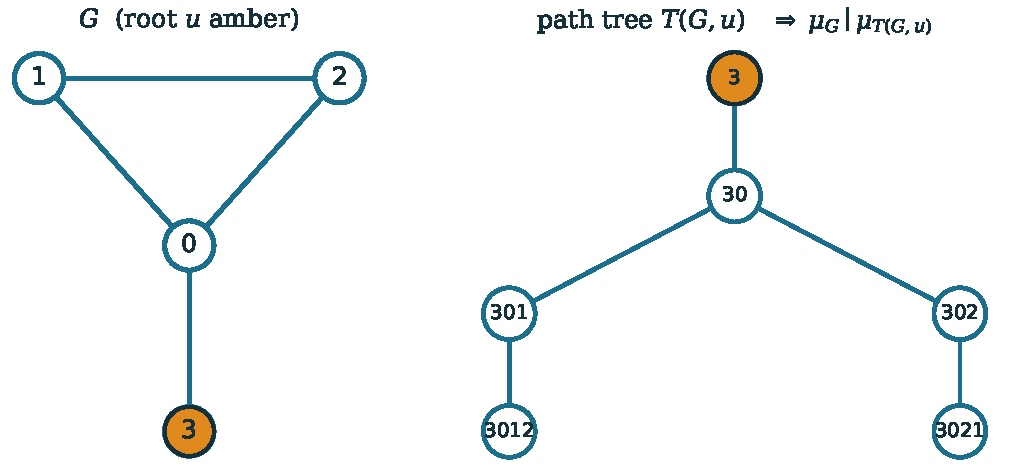
\includegraphics[width=0.96\textwidth]{fig2_pathtree.pdf}
  \caption{Unfolding the ``paw'' graph $G$ (left, root $u$ amber) into its path
  tree $T(G,u)$ (right): each vertex of $T$ is a vertex-simple path of $G$ from
  $u$, written as its vertex sequence; two are joined when one extends the other
  by an edge. $T(G,u)$ is acyclic (Theorem~\ref{thm:acyclic}), and $\mu_G$ divides
  $\mu_{T(G,u)}$ (Section~\ref{sec:divis}).}
  \label{fig:pathtree}
\end{figure}

% ===============================================================
\section{Fact (ii): forests are gauge-trivial}
\label{sec:forest}

Why is a tree the easy case? Because on it the matching polynomial loses its
combinatorial character and becomes a spectral object.

\begin{theorem}[Forest identity]
\label{thm:forest}
For an acyclic graph $F$,
\keyeq{\mu_F \;=\; \operatorname{charpoly}(A_F)\qquad
  (\lean{matchingPoly\_forest\_eq\_charpoly}),}
the characteristic polynomial of the (real, symmetric) adjacency matrix.
\end{theorem}

The proof is the permutation expansion of $\det(xI-A_F)$. A permutation
contributes only through its support; on a forest, the support of any
contributing permutation decomposes into transpositions along edges---the
\emph{forest-involution lemma} (\lean{acyclic\_perm\_support\_isInvolution}): any
permutation whose every non-fixed point is adjacent to its image is an involution,
because a longer orbit would close a cycle. The surviving terms are exactly the
matchings, with the right signs, reassembling $\mu_F$. Since $A_F$ is real
symmetric, the spectral theorem gives a real spectrum
(\lean{charpoly\_symmetric\_realRooted}): $\mu_F$ is real-rooted. The harder
spectral fact---that the roots lie in the band---is the whole of
Sections~\ref{sec:gershgorin}--\ref{sec:weight}.

% ===============================================================
\section{Fact (i): divisibility, and the wall I crossed}
\label{sec:divis}

A tree is easy, but the polynomial I care about lives on $G$, not on $T(G,u)$. So
the sharp question is: \emph{why should the matching polynomial of an arbitrary
graph---cycles and all---divide that of a tree built from its paths?} The forest
identity makes the tree easy; the divisibility makes it \emph{relevant}.

\begin{theorem}[Divisibility]
\label{thm:divis}
For a connected graph $G$ and vertex $u$,
\keyeq{\mu_G \;\bigm|\; \mu_{T(G,u)}\qquad
  (\lean{connected\_matchingPoly\_dvd\_pathTree}).}
\end{theorem}

Mathematically this is Godsil's induction on the vertex-deletion recurrence of the
matching polynomial,
\keyeq{\mu_G \;=\; x\,\mu_{G-v}\;-\;\sum_{u\sim v}\mu_{G-v-u}
  \qquad(\lean{matchingPoly\_recurrence}),}
applied at $u$ in $G$ and at the root $r$ in $T$, and combined through
\emph{Godsil's identity}
\keyeq{\mu_G\,\mu_{T(G,u)-r}\;=\;\mu_{G-u}\,\mu_{T(G,u)},}
which, with the root-decomposition of the path tree, yields the divisibility. (The
formalization carries the recurrence in its $x^2$-cleared form, with each deletion
isolating a vertex, to keep the vertex count fixed.) What is worth reporting is the
last step, because it is where an earlier draft of this paper stopped.

\paragraph{The wall.} The path tree lives on a dependent $\Sigma$-of-paths type.
Specializing the general divisibility to a concrete graph requires Lean to compare
the matching polynomial computed with one \lean{Fintype}/\lean{DecidableRel}
instance against the same polynomial computed with another; the two are
\emph{equal} (the polynomial does not depend on these subsingleton instances), but
asking \lean{isDefEq} to see it forces a \lean{whnf} reduction of $\mu$ over the
path type, and the heartbeat budget is exhausted. The draft diagnosed this as an
\emph{elaboration} wall, not a mathematical gap, and stopped there.

\paragraph{The crossing.} The cure is to transport the \emph{hypothesis} to the
local instances rather than the goal to the foreign ones. With the
instance-irrelevance lemma \lean{matchingPoly\_inst\_irrel} (proved by
\lean{Subsingleton.elim}, not \lean{congr}, precisely to avoid the \lean{whnf}),
one rewrites each occurrence of $\mu(T(G,u))$ with the \emph{graph head pinned},
making the rewrite a keyed, syntactic match that never reduces $\mu$. Four such
rewrites close the theorem; \lean{\#print axioms} reports no \lean{sorryAx}. The
lesson the draft could only conjecture is now confirmed in code: the wall was
instance divergence, and pinning the head dissolves it.

% ===============================================================
\section{Real-rootedness, assembled}
\label{sec:realrooted}

The divisibility (Theorem~\ref{thm:divis}) needs $G$ connected; \emph{does
real-rootedness?} It does not---and the gap is exactly the disjoint union, which
the matching polynomial handles by multiplying. With the two facts in hand,
real-rootedness is short. A nonzero divisor of a polynomial that splits over $\R$
also splits (\lean{RealRooted.of\_dvd}, wrapping
\lean{Polynomial.Splits.of\_dvd}). The path tree is a forest
(Theorem~\ref{thm:acyclic}), so $\mu_{T(G,u)}$ is a characteristic polynomial of a
symmetric matrix, hence splits (Theorem~\ref{thm:forest}); therefore its divisor
$\mu_G$ splits too---$\mu_G$ is real-rooted for connected $G$
(\lean{matchingPoly\_connected\_realRooted}). A general graph is the disjoint union
of its components and $\mu$ is multiplicative over components
(\lean{matchingPoly\_eq\_prod\_components}); each induced component is connected
(\lean{maximal\_connected\_induce\_supp}), and real-rootedness multiplies. This is
\lean{matchingPoly\_realRooted}, for every finite graph.

% ===============================================================
\section{The bound, half one: a weighted Gershgorin estimate}
\label{sec:gershgorin}

Real-rootedness says the roots are real; the bound says none exceeds a ceiling
fixed by the degree alone. Where does a degree-only ceiling on the largest
eigenvalue of a symmetric matrix come from?

The tool is a \emph{weighted} Gershgorin estimate---the Collatz--Wielandt
direction of Perron--Frobenius, stated for one eigenvalue and proved by hand so no
positivity theory is needed.

\begin{theorem}[Weighted Gershgorin]
\label{thm:cw}
Let $A$ be a square real matrix with nonnegative entries and $w$ a strictly
positive vector with $\sum_j A_{ij}\,w_j\le B\,w_i$ for all $i$. Then every real
root $\mu$ of $\operatorname{charpoly}(A)$ satisfies
\keyeq{|\mu|\;\le\;B\qquad(\lean{collatzWielandt}).}
\end{theorem}

The proof is the eigenvector argmax argument, and it is short enough to give in
full. A root of the characteristic polynomial gives, through $\det(\mu I-A)=0$ and
\lean{Matrix.exists\_mulVec\_eq\_zero\_iff}, an eigenvector $v\ne0$ with $Av=\mu
v$. Pick the coordinate $k$ that maximizes $|v_j|/w_j$. Then, using $A_{kj}\ge0$
and $|v_j|/w_j\le|v_k|/w_k$,
\[
  |\mu|\,|v_k|
  =\Bigl|\sum_j A_{kj}v_j\Bigr|
  \le\sum_j A_{kj}\,w_j\frac{|v_j|}{w_j}
  \le\Bigl(\sum_j A_{kj}w_j\Bigr)\frac{|v_k|}{w_k}
  \le B\,w_k\frac{|v_k|}{w_k}=B\,|v_k|,
\]
and $|v_k|>0$. This is the entire analytic engine of the bound. Gluing it to the
matching polynomial is one lemma (\lean{forest\_bounded\_of\_weight}): on a forest,
$A_F$ is symmetric and nonnegative (its entries are $0/1$) and $\mu_F$ is its
characteristic polynomial (Theorem~\ref{thm:forest}), so Theorem~\ref{thm:cw}
bounds the roots---\emph{once I exhibit a weight whose weighted row sums are
$\le 2\sqrt{\Delta-1}$}.

% ===============================================================
\section{The bound, half two: a weight and two tree facts}
\label{sec:weight}

What weight forces the row sums down to exactly $2\sqrt{\Delta-1}$? On a tree,
rooted at one vertex per component, give each vertex a weight that decays
geometrically with its distance from the root:
\keyeq{w_v\;=\;\bigl(\sqrt{\Delta-1}\bigr)^{-\operatorname{dist}(r,v)}.}
The arithmetic of why this works is the content of Figure~\ref{fig:weight}. Write
$s=\sqrt{\Delta-1}$ and $q=\Delta-1$. A neighbour one step \emph{closer} to the
root contributes $w_v\cdot s$; one step \emph{farther} contributes $w_v/s$. So
with $a$ closer neighbours and $b$ farther ones,
\[
  \sum_{u\sim v}w_u \;=\; w_v\Bigl(a\,s+\tfrac{b}{s}\Bigr),
\]
and the bound $a\,s+b/s\le 2s$ reduces, after multiplying by $s$ and using
$s^2=q$, to a single integer inequality:
\keyeq{a\,q+b\;\le\;2q,\qquad\text{i.e.}\qquad (\Delta-2)(1-a)\ge0,}
which holds with $a\le1$ (Fact~2 below), $a+b\le\Delta$ (the degree bound), and
$\Delta\ge2$. This last arithmetic is isolated as \lean{rowsum\_arith}, and it is
where the hypothesis $\Delta\ge2$ earns its place.

\begin{figure}[t]
  \centering
  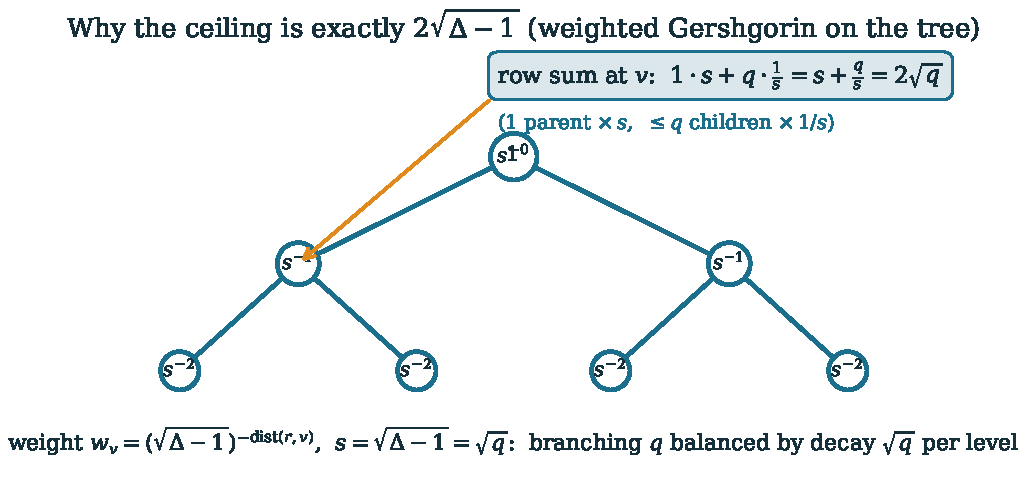
\includegraphics[width=0.92\textwidth]{fig3_weight.pdf}
  \caption{Why the ceiling is exactly $2\sqrt{\Delta-1}$. With the geometric weight
  $w_v=(\sqrt{\Delta-1})^{-\operatorname{dist}(r,v)}$, the weighted row sum at a
  vertex $v$ balances its one parent (heavier by $s=\sqrt{q}$) against its
  $\le q$ children (lighter by $s$), giving $s+q/s=2\sqrt{q}$. The branching
  factor $q$ is exactly cancelled by a $\sqrt{q}$ decay per level.}
  \label{fig:weight}
\end{figure}

The two structural inputs that the row-sum computation consumes are the only graph
theory the bound really needs. Both are facts about distances from the root in a
tree.

\begin{theorem}[Fact 1: neighbours differ by exactly one]
\label{thm:f1}
In an acyclic graph with root $\rho$, for an edge $u\sim v$ with $u$ reachable
from $\rho$,
$\operatorname{dist}(\rho,u)=\operatorname{dist}(\rho,v)\pm1$
(\lean{forest\_adj\_dist\_pm\_one}).
\end{theorem}

The $\le1$ half is the triangle inequality: a shortest path to one endpoint,
extended by the edge, reaches the other. The $\ne$ half is bipartiteness. A tree
is bipartite (\lean{IsAcyclic.isBipartite}), so a two-colouring $c$ exists; on a
shortest path, $c$ records the parity of its length
(\lean{Coloring.even\_length\_iff\_congr}), so the colour of a vertex is the parity
of its distance from $\rho$. Adjacent vertices have different colours
(\lean{Coloring.valid}), hence different parities, hence different distances.

\begin{theorem}[Fact 2: at most one parent]
\label{thm:f2}
In an acyclic graph, at most one neighbour of $v$ is one step closer to the root
(\lean{forest\_le\_one\_parent}).
\end{theorem}

Two such neighbours would give two shortest paths $\rho\to v$ ending in different
last edges; in a tree the path between two vertices is unique
(\lean{IsAcyclic.path\_unique}), and \lean{IsPath.eq\_penultimate\_of\_mem\_edges}
pins both candidates to the single penultimate vertex of that path, so they
coincide. (A shortest walk is a path---via \lean{bypass}---supplies the shortest
paths: \lean{exists\_isPath\_length\_eq\_dist}.)

Assembling the weight, the two facts, and the arithmetic gives the forest bound
(\lean{forest\_bounded\_proof}): \emph{the matching polynomial of a forest of
maximum degree $\le\Delta$ has all roots in
$[-2\sqrt{\Delta-1},2\sqrt{\Delta-1}]$.} Because $\mu_F=\operatorname{charpoly}$,
this is exactly the classical statement that a tree of maximum degree $\Delta$ has
spectral radius $\le2\sqrt{\Delta-1}$ (Godsil; Stevanovi\'c~\cite{Stevanovic2003})
---now, to my knowledge, first checked by a machine.

\paragraph{A sharper, local weight.} The weight above uses the global $\Delta$. A
purely \emph{local} choice---multiply by $1/\sqrt{d_{\text{parent}}-1}$ at each
step down from the root---telescopes to the per-edge bound
$\sqrt{d_u-1}+\sqrt{d_v-1}$, strictly sharper on irregular trees and recovering
$2\sqrt{\Delta-1}$ in the regular case (confirmed numerically before formalizing).
It is the cleaner object---defined edge-locally, needing no global depth---and is
the form the development uses. I do not claim the local bound as new mathematics:
degree-sequence spectral bounds for trees are well studied; the contribution is
the machine-checked statement.

\paragraph{The boundary, stated honestly.} The hypothesis $\Delta\ge2$ is not
cosmetic. At $\Delta=1$ the band $2\sqrt{\Delta-1}$ collapses to $\{0\}$, yet a
single edge $K_2$ has $\mu_{K_2}=x^2-1$ with roots $\pm1$. (For $\Delta\le1$ a
graph is a matching, with roots in $\{-1,0,1\}$.) This is the standard
Heilmann--Lieb hypothesis; I flag it because I only noticed it by testing the
boundary case, and an honest formalization must say where its statement is false.

% ===============================================================
\section{Assembly: from the tree to every graph}
\label{sec:assembly}

The bound now holds on $T(G,u)$---a graph whose vertices are \emph{paths}, not the
vertices of $G$. \emph{What stands between that bound and the one I want on $G$?}
Three short steps, and they are exactly the gap.

\textbf{The path tree is not too bushy} (\lean{pathTree\_degree\_le}): $T(G,u)$ has
maximum degree $\le\Delta_G$. The map ``a path-tree neighbour $\mapsto$ its
endpoint'' injects the neighbours of a node $p$ into the $G$-neighbours of $p$'s
endpoint; injectivity is the path-tree structure---children are determined by their
endpoint, the parent is unique, and a child and the parent cannot share an
endpoint (the child's is off $p$'s support, the parent's is on it).

\textbf{Transfer} (\lean{connected\_matchingPoly\_bounded}): by
Theorem~\ref{thm:divis}, $\mu_G\mid\mu_{T(G,u)}$, and the path tree is a forest of
degree $\le\Delta$, so its matching polynomial is banded
(\lean{forest\_bounded\_proof}); a nonzero divisor of a banded polynomial is banded
(\lean{BoundedBy.of\_dvd}). The transfer meets the same $\Sigma$-paths
\lean{whnf} wall as the divisibility, and the same \lean{matchingPoly\_inst\_irrel}
surgery dissolves it---this time the build finishes with no timeout.

\textbf{General} (\lean{matchingPoly\_bounded}): over connected components
(\lean{BoundedBy.prod}), with each induced component connected and of degree
$\le\Delta$---its $G$-neighbours stay inside the component, so
\lean{degree\_induce\_of\_neighborSet\_subset} gives equality. This is the bound
of Theorem~\ref{thm:HL}. Figure~\ref{fig:nested} shows the chain of containments
the proof realizes; Table~\ref{tab:numeric} confirms the endpoint numerically.

\begin{figure}[t]
  \centering
  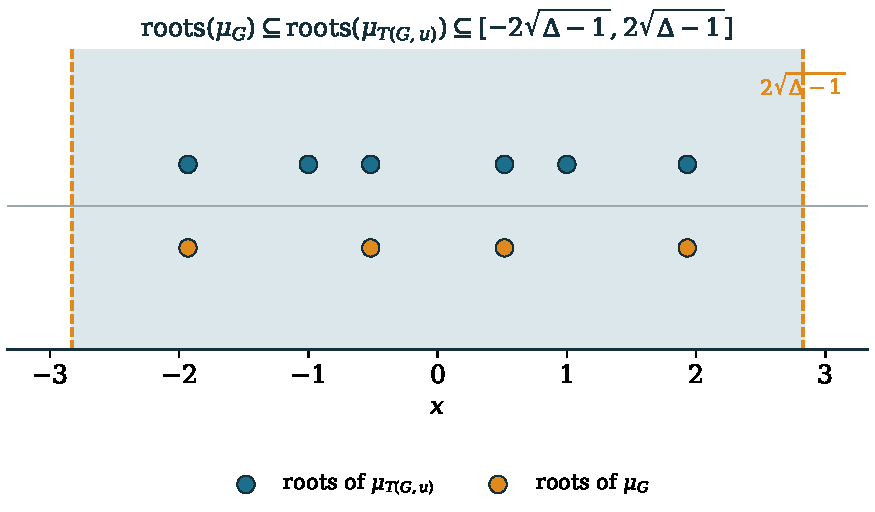
\includegraphics[width=0.88\textwidth]{fig4_nested.pdf}
  \caption{The proof in one line of reasoning, on the paw graph: the roots of
  $\mu_G$ are a subset of the roots of $\mu_{T(G,u)}$ (because $\mu_G\mid
  \mu_{T(G,u)}$), which lie in the band (because $T(G,u)$ is a forest). Hence the
  roots of $\mu_G$ lie in the band.}
  \label{fig:nested}
\end{figure}

% ===============================================================
\section{Why one construction gives both halves}
\label{sec:duality}

Real-rootedness and the bound look like two theorems---one about reality, one about
magnitude. \emph{Why does a single tree settle both at once?} A short thread
explains it, and it ties this paper to the Ihara-zeta side of the same program. Consider the ratio $R(G,a)=\mu_{G-a}/\mu_G$, the matching polynomial's
Green's function. Dividing the deletion recurrence by $\mu_{G-a}$ turns it into a
continued fraction $1/R_a=x-\sum_{b\sim a}R_b$; on the $(q{+}1)$-regular tree this
is self-consistent and solves $qR^2-xR+1=0$, whose branch is $R=1/u$ with $u$ the
Ihara non-backtracking variable. The spectral and zeta variables are tied by the
Joukowski map
\keyeq{\lambda \;=\; u+\frac{q}{u}\;=\;q\,R+\frac1R ,\qquad q=\Delta-1.}
On the critical circle $|u|=1/\sqrt{q}$ this reads $\lambda=2\sqrt{q}\,\cos\theta$:
the band $[-2\sqrt{q},2\sqrt{q}]$ is precisely the \emph{shadow} of the critical
circle under Joukowski, a two-to-one projection identifying conjugate pairs
$u,\bar u$ (Figure~\ref{fig:joukowski}). Real-rootedness of $\mu_G$ is the
statement that $R$ is a Stieltjes function; the bound is the location of its branch
cut. I verified the algebra symbolically and claim none of it as new (it is the
Bethe-lattice / Kesten--McKay Green's function meeting the Ihara--Bass picture);
it is the reason the path tree and the graph zeta function, formalized in the same
repository, are two readings of one variable.

\begin{figure}[t]
  \centering
  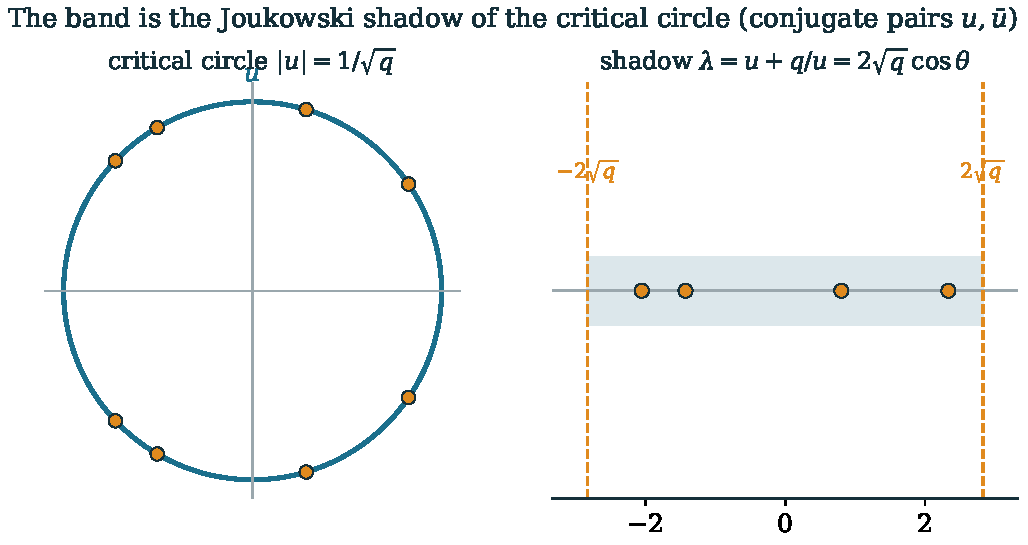
\includegraphics[width=0.92\textwidth]{fig5_joukowski.pdf}
  \caption{The band is the Joukowski shadow of the critical circle. Points
  $u,\bar u$ on the circle $|u|=1/\sqrt{q}$ (left) project to a single real
  $\lambda=u+q/u=2\sqrt{q}\cos\theta$ in the band $[-2\sqrt{q},2\sqrt{q}]$ (right).
  The two-to-one identification of conjugates is the Ihara-zeta functional
  equation in disguise.}
  \label{fig:joukowski}
\end{figure}

% ===============================================================
\section{What the theorem is for, and what it is not}
\label{sec:context}

A machine-checked theorem earns a blunt question: \emph{what can it do that the
informal theorem could not, and where does its reach end?} Heilmann--Lieb is the
analytic input to the Marcus--Spielman--Srivastava proof that bipartite Ramanujan
graphs of every degree exist~\cite{MSS2015a}. Their argument
needs two facts about the expected characteristic polynomial of a random $\pm1$
edge signing: that it equals $\mu_G$ (Godsil--Gutman, Paper~I), and that its roots
lie in the band (Theorem~\ref{thm:HL}). \emph{Both are now formalized}
(Figure~\ref{fig:interlacing}). What is not
here is the interlacing-families existence step, nor the signing/$2$-lift
correspondence; those remain future work, and I claim nothing about them.

\begin{figure}[t]
  \centering
  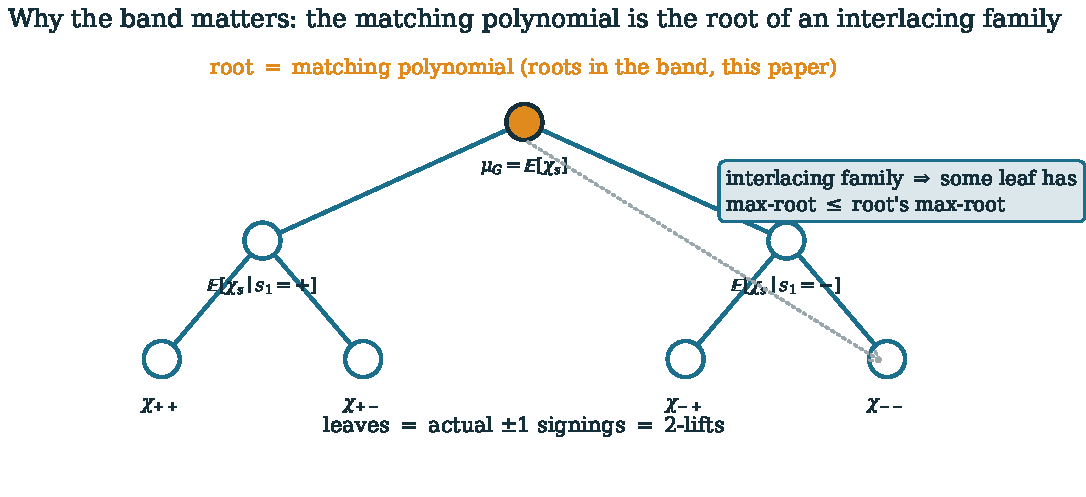
\includegraphics[width=0.86\textwidth]{fig7_interlacing.pdf}
  \caption{Where this theorem sits in the Marcus--Spielman--Srivastava argument.
  Fixing the edge signs one at a time builds a binary tree of conditional expected
  characteristic polynomials; its root is the matching polynomial---whose roots
  this paper confines to the band---and its leaves are the actual $\pm1$ signings,
  i.e.\ the $2$-lifts. Because the polynomials form an \emph{interlacing family},
  some leaf has its largest root no larger than the root's: a bounded average forces
  a good individual. This paper certifies the root; the tree itself is future work
  (Q1).}
  \label{fig:interlacing}
\end{figure}

In
particular this paper formalizes Heilmann--Lieb, not the existence of Ramanujan
graphs.

I also asked, honestly and with exact computation, whether anything in this
framework gives purchase on the \emph{open} problem of non-bipartite Ramanujan
graphs of all degrees~\cite{LevinSurvey}. It does not, and the obstruction is
mechanical. The interlacing method controls one end of the spectrum because the
expected polynomial $\mathbb{E}[\operatorname{charpoly}(A_s)]=\mu_G$ is real-rooted.
The natural two-sided handle would be
$\mathbb{E}[\operatorname{charpoly}(A_s^2)]$, whose largest root would control
$\max_i|\lambda_i|$---but a direct symbolic check shows this average is \emph{not}
real-rooted in general (it has, for instance, zero real roots for $K_{3,3}$). The
linearity that makes the matching polynomial special does not survive squaring. I
report this as a negative result: there is no easy crack here, consistent with the
problem's reputation.

% ===============================================================
\section{Implications}
\label{sec:implications}

\emph{Beyond the theorem itself, what does this proof leave behind for someone
else to use?}

\paragraph{Reusable, certified blocks.} New to Mathlib and not matching-specific:
\lean{collatzWielandt}, a hands-on weighted Gershgorin eigenvalue bound built from
the ingredients of \lean{Matrix.eigenvalue\_mem\_ball}; the \lean{BoundedBy}
predicate with divisor- and product-closure and \lean{RealRooted.of\_dvd}; and two
clean tree-distance facts---neighbours differ in root-distance by one (via
bipartiteness), at most one neighbour is closer (via path-uniqueness)---that any
rooted-tree argument over \lean{SimpleGraph} can reuse.

\paragraph{Reach across fields, and how the artifact serves each.} Heilmann--Lieb
sits at a crossroads, and a verified version is useful differently on each road.
\emph{Statistical mechanics / mathematical physics}: $\mu_G$ is the monomer--dimer
partition function, and the band is a zero-free region of it; the formalization is
a machine-checked foundation for Lee--Yang-style analyticity arguments (free energy
without phase transition) on bounded-degree lattices. \emph{Spectral graph theory
and theoretical computer science}: the theorem is the analytic engine behind
Ramanujan graphs, expanders, derandomization and error-correcting codes; with the
Godsil--Gutman identity (Paper~I) it gives the two verified inputs an expander
existence proof needs, and a concrete stepping stone toward a formalized
Marcus--Spielman--Srivastava (Q1). \emph{Algebraic combinatorics}: the reusable
real-rootedness and \lean{BoundedBy} infrastructure---divisor- and product-closed,
fed by interlacing-free spectral bounds---applies to any real-rooted-polynomial
question (log-concavity of the $m_k$, stable polynomials). \emph{Formal mathematics}:
the matching polynomial, the path tree, a weighted Gershgorin eigenvalue bound, and
two tree-distance lemmas are new, Mathlib-grade, and contributable upstream, where
they lower the cost of the next spectral or combinatorial formalization.
\emph{Number theory, by analogy}: through the duality of
Section~\ref{sec:duality} the same repository holds the Ihara-zeta / graph-Riemann
side, so the artifact is also a substrate for a unified, formalized graph RH (Q5).

\paragraph{Completing the path-tree program.} Together with Paper~I, the matching
polynomial, the Godsil--Gutman identity, the path tree, real-rootedness and the
root bound are now machine-checked. No proof assistant, to my knowledge, had the
matching polynomial or either half of Heilmann--Lieb before this line of work; the
``first'' claim is supported by a search of the Lean/Mathlib, Isabelle/AFP and
Coq/mathcomp ecosystems (see the honesty caveat in Section~\ref{sec:intro}), and
the mathematics is entirely classical.

% ===============================================================
\section{Methodology}
\label{sec:method}

\emph{What did building this proof teach about how to build such proofs?}
As in Paper~I, I ran a build-as-oracle loop with an AI system (Claude, Anthropic):
it proposed the definitions and proofs, the Lean kernel verified or rejected each,
and I sized the write-up to the kernel's verdict. To be precise about the division
of labour, since it is fair to ask: the assistant proposed essentially all of the
Lean definitions and proof scripts and a first draft of this text, while I set the
goal and the route, made the design decisions (the path-tree choice, the local
weight, the diagnosis of the elaboration wall), checked every statement against the
intended mathematics, and take responsibility for all claims. Correctness here does
not rest on trust in the assistant: the Lean kernel verified every line, a proof it
rejects never enters the paper, and the non-vacuity of the statements is witnessed
by \lean{\#print axioms} (Appendix~\ref{sec:formal}). The assistant proposes; the
kernel disposes. Two
practices were decisive. First, the route to the bound was \emph{de-risked
numerically before any Lean}: a short SageMath study settled which inductive
invariant closes (a flat per-vertex ratio fails on graphs with cycles; the
rooted-tree weight closes exactly at the band edge), so the formalization pursued a
route already known to work---the local weight of Section~\ref{sec:weight} arose
this way. Second, after the proof was complete I applied the same falsification
discipline \emph{to my own conclusions}, deliberately hunting for a new theorem in
the neighbourhood, and report the honest outcome of Section~\ref{sec:context}: the
territory is classical and occupied, and the one promising probe was killed by a
computation. The contribution is a verified formalization, stated to the exact
boundary of what the kernel checked, with the negatives reported as plainly as the
positives.

% ===============================================================
\section{Related work}
\label{sec:related}

The mathematics is classical. Heilmann--Lieb~\cite{HeilmannLieb1972} is the target;
the path-tree route and the forest spectral bound are Godsil's
~\cite{Godsil1981Matchings,Godsil1993}, with the elementary tree spectral-radius
bound also in Stevanovi\'c~\cite{Stevanovic2003}; the theorem is the analytic half
of Marcus--Spielman--Srivastava~\cite{MSS2015a}; the Green's-function picture of
Section~\ref{sec:duality} is Abert--Csikvari--Frenkel--Kun~\cite{AbertCsikvariFrenkelKun2016}
and its Ihara-zeta face is Terras~\cite{Terras2011}. On the formalization side,
Mathlib~\cite{Mathlib2020} provides simple graphs, walks, paths, the
characteristic polynomial, the Hermitian spectral theorem, and Gershgorin's circle
theorem, but not the matching polynomial (Paper~I), the path tree, or a
\lean{BoundedBy} / weighted-Gershgorin matching bound (this paper). I am aware of
no prior machine-checked treatment of Heilmann--Lieb.

% ===============================================================
\section{Questions left open}
\label{sec:open}

A formalization is only as alive as the questions it makes askable next. I leave
six, ordered from the most reachable to the most speculative; each names a tension
I could not resolve here.

\begin{enumerate}\itemsep3pt
\item[\textbf{Q1}] \emph{(The next stone.)} The two analytic inputs to
  Marcus--Spielman--Srivastava are now formalized---the expected signed
  characteristic polynomial \emph{is} $\mu_G$ (Paper~I) and its roots lie in the
  band (this paper). What is the \emph{smallest} further step that yields the first
  machine-checked proof that bipartite Ramanujan graphs of every degree exist---the
  interlacing-families existence argument, or the signing/$2$-lift correspondence?
\item[\textbf{Q2}] \emph{(The hardest.)} I showed the obvious two-sided handle
  $\mathbb{E}[\operatorname{charpoly}(A_s^2)]$ is not real-rooted. Is there
  \emph{any} polynomial, linear in a random combinatorial structure, whose largest
  root controls $\max_i|\lambda_i|$ and stays real-rooted? A ``yes'' is a route into
  the open non-bipartite Ramanujan problem; this paper proves only that the naive
  candidate is a ``no''.
\item[\textbf{Q3}] \emph{(Local sharpness.)} The edge-local weight gives the
  per-edge bound $\sqrt{d_u-1}+\sqrt{d_v-1}$, strictly better than $2\sqrt{\Delta-1}$
  on irregular trees. Does that sharpness translate into a useful statement about
  irregular graphs---an irregular expansion threshold, or an irregular analogue of
  the graph Riemann hypothesis through the $Q=D-I$ Ihara--Bass picture?
\item[\textbf{Q4}] \emph{(Cheap, not just survivable.)} The $\Sigma$-paths
  elaboration wall was crossed by an instance-irrelevance surgery, but the cost is
  still there. Can $\mu$'s isomorphism-invariance be reproved \lean{whnf}-free (via
  its edge-set bijection rather than a per-degree matching count), making the
  path-tree machinery cheap for any future development?
\item[\textbf{Q5}] \emph{(One variable, one theorem.)} The duality $u=1/R$ puts the
  matching side and the Ihara-zeta side on a single uniformizing variable, sharing
  the \lean{BoundedBy} substrate in one repository. Is there a single formalized
  statement from which both the Ramanujan band (matching) and the graph Riemann
  hypothesis (zeta) fall out as readings?
\item[\textbf{Q6}] \emph{(For the physicist.)} $\mu_G$ is the monomer--dimer
  partition function, and the band is a zero-free region of it. Does the
  machine-checked real-rootedness and band have a consequence a statistical
  physicist would want---analyticity of the free energy, an absence-of-phase-%
  transition statement in the Lee--Yang spirit---that is now itself
  machine-checkable?
\end{enumerate}

% ===============================================================
\section{Conclusion}

Paper~I asked how a real-rootedness statement about an arbitrary graph could be
machine-checked, proposed Godsil's path tree as the answer, and left it as an
explicit invitation. This paper accepts the invitation and finishes the job: it
builds the path tree, proves the forest identity and the divisibility---crossing
the single elaboration wall that had stopped the draft---and proves the Ramanujan
bound from a weighted Gershgorin estimate fed by a geometric tree weight and two
facts about distances in a tree. The result is the Heilmann--Lieb theorem, both
halves, \lean{sorry}-free, to the exact boundary $\Delta\ge2$ where it holds. None
of the mathematics is new; the contribution is that it is now verified where I
could find no prior formalization, and that the stone named at the end of Paper~I
is laid.

And the journey ends where it began: with a single number. The quantity
$2\sqrt{\Delta-1}$ first marked the edge of analyticity of a lattice gas; it
reappeared as the spectral radius of an infinite tree, then named the Ramanujan
graphs, then ruled the critical line of a graph's zeta function. This paper records,
in a form a machine has checked from the axioms up, that the same number also bounds
the matchings of every finite graph. One number, four times over---and, for this
last reading, now beyond doubt.

\paragraph{Artifacts and reproducibility.} All Lean sources are \lean{sorry}-free
and depend only on the three standard axioms (Appendix~\ref{sec:formal},
Table~\ref{tab:results}). The build uses toolchain
\lean{leanprover/lean4:v4.30.0-rc2} against a Mathlib clone; \lean{lake build MSS}
checks the development (exit~0), and the non-vacuity of each headline theorem is
reproduced by a three-line file---\lean{import MSS.HeilmannLiebBound};
\lean{open SimpleGraph}; \lean{\#print axioms matchingPoly\_bounded}---run under
\lean{lake env lean}. The exact snapshot accompanying this paper is pinned by its
Zenodo DOI; the sources and the SageMath cross-checks are at:
\begin{center}
\url{https://github.com/karlesmarin/godsil-gutman-lean}
\end{center}

% ===============================================================
\appendix
\section{Formal statements, verbatim}
\label{sec:formal}

\emph{Does the Lean statement say the theorem, or something weaker?} That is the
first question a careful reader of a formalization should ask, and it deserves a
direct answer. Below are the load-bearing definitions and the two headline
signatures, transcribed from the source (identifiers in typewriter font, the
Unicode operators rendered in mathematics). Real-rootedness is splitting over
$\R$; the band predicate is real-rootedness \emph{and} the magnitude bound on every
root---so the conclusions are the genuine statements, not weakenings.

\begin{tcolorbox}[colframe=ggteal,colback=ggband!25,arc=2pt,boxrule=0.8pt,left=8pt,right=8pt]
\ttfamily\small\setlength{\parindent}{0pt}
def RealRooted (p : Polynomial $\R$) : Prop := p.Splits\\[2pt]
def BoundedBy (p : Polynomial $\R$) (B : $\R$) : Prop :=\\
\hspace*{1.5em}RealRooted p $\wedge$ $\forall$ x : $\R$, p.IsRoot x $\rightarrow$ |x| $\leq$ B\\[2pt]
def bruhatTitsBound (k : $\mathbb{N}$) : $\R$ := 2 * Real.sqrt (k - 1 : $\R$)\\[4pt]
def matchingPoly : Polynomial $\R$ :=\\
\hspace*{1.5em}$\sum$ k $\in$ Finset.range (Fintype.card V / 2 + 1),\\
\hspace*{3em}Polynomial.C ((-1 : $\R$)\^{}k * (G.matchingNumber k : $\R$))\\
\hspace*{3em}* Polynomial.X\^{}(Fintype.card V - 2 * k)\\[6pt]
theorem matchingPoly\_realRooted (G : SimpleGraph V) [DecidableRel G.Adj] :\\
\hspace*{1.5em}MSS.RealRooted G.matchingPoly\\[4pt]
theorem matchingPoly\_bounded (G : SimpleGraph V) [DecidableRel G.Adj] ($\Delta$ : $\mathbb{N}$)\\
\hspace*{1.5em}(h$\Delta$ : 2 $\leq$ $\Delta$) (hdeg : $\forall$ v, G.degree v $\leq$ $\Delta$) :\\
\hspace*{1.5em}BoundedBy G.matchingPoly (bruhatTitsBound $\Delta$)
\end{tcolorbox}

\noindent Neither theorem is vacuous. A statement of the shape
``$\dots\lor\mathrm{True}$'' would also be \lean{sorry}-free, so absence of
\lean{sorry} is necessary but not sufficient; it is the \emph{explicit} conclusions
above---\lean{RealRooted} and \lean{BoundedBy} with the definitions shown---that
rule vacuity out. For each headline theorem, \lean{\#print axioms} returns exactly
\lean{[propext, Classical.choice, Quot.sound]} (no \lean{sorryAx}), and the full
\lean{MSS} library builds (\lean{lake build MSS}, exit~0) under toolchain
\lean{leanprover/lean4:v4.30.0-rc2} against a local Mathlib clone.

\bibliographystyle{plain}
\bibliography{references}

\end{document}
